\documentclass{checkpoint/llncs}

\usepackage[italian]{babel}
\usepackage[utf8]{inputenc}
%% \usepackage[english]{babel}
\usepackage[T1]{fontenc}
\usepackage{blindtext}
\usepackage{amsmath}
\usepackage{amssymb}
\usepackage{amsmath}
\usepackage{graphicx}
\usepackage{mathtools}
\usepackage{listings}
\usepackage[dvipsnames]{xcolor}
\usepackage[normalem]{ulem}
\usepackage{listings}
\usepackage[export]{adjustbox}
\usepackage{lscape}
\usepackage{float}
\usepackage{booktabs}

\usepackage{pdftricks}
\begin{psinputs}
  \usepackage{pstricks}
\end{psinputs}
\usepackage[pdf]{pstricks}

\usepackage{float}
\usepackage[hypertexnames=false]{hyperref}
\usepackage{algorithm}
\usepackage[noend]{algpseudocode}
\floatname{algorithm}{Algoritmo}
\renewcommand{\algorithmicrequire}{\textbf{Precondizioni:}}

\usepackage{cleveref}
\usepackage{tikz}
\usetikzlibrary{matrix,shapes,arrows,positioning,chains}
\usepackage{hhline}
\usepackage{multirow}

\pagestyle{plain}

%%%%
\newcommand*{\sst}{\mathrel{|}}
\newcommand*{\nohyp}{\phantom{x}}
\providecommand*{\Nset}{\mathbb{N}}
\providecommand*{\Vset}{\mathbb{V}}
\providecommand*{\Sset}{\mathbb{S}}
\newcommand*{\fund}[3]{\mathord{#1}\colon#2\rightarrow#3}
\newcommand{\defrel}[1]{\mathrel{\buildrel \mathrm{def} \over {#1}}}
\newcommand{\defeq}{\defrel{=}}
\newcommand*{\sseq}{\subseteq}
\newcommand*{\sqsseq}{\sqsubseteq}
\newcommand*{\cR}{\ensuremath{\mathcal{R}}}
\newcommand*{\cG}{\ensuremath{\mathcal{G}}}
\newcommand*{\cV}{\ensuremath{\mathcal{V}}}
\newcommand*{\cQ}{\ensuremath{\mathcal{Q}}}
\newcommand{\sset}[2]{{\renewcommand{\arraystretch}{1.2}
                      \left\{\,#1 \,\left|\,
                               \begin{array}{@{}l@{}}#2\end{array}
                                 \right.   \,\right\}}}
\newcommand*{\oneg}[1]{\overline{#1}}
\renewcommand*{\iff}{\mathrel{\Leftrightarrow}}
\newcommand*{\ifff}{\mathrel{\Longleftrightarrow}}
\newcommand*{\nmod}{\nvDash}
\newcommand*{\densem}[1]{\ensuremath{\rrbracket #1 \llbracket}}
\newcommand*{\view}{\mathrm{view}}
\newcommand*{\adj}[2]{\mathrm{adj}_{#2}(#1)}
\newcommand*{\printlog}[1]{\ \ \begin{footnotesize}\texttt{#1}\end{footnotesize}}
%%%%%%%%%%%%%%%%%%%%%%%%%%%%%%%%%%%%%%%%%%%%%%%%%%%%%%%%%
\newcommand*{\coanote}[1]{\textbf{Coauthor note}: #1}
\newcommand*{\coafootnote}[1]{\footnote{\extbf{Coauthot note}: #1}}

%%%%
\title{A distribuited algorithm\\for the subgraph isomorphism problem}

\author{Anna Becchi, matr. 140603\\
  Idriss Riouak, matr. 13????}
\institute{Laurea Magistrale in Informatica\\Universit\`a di Udine}
\date{A.A. 2017/2018}
%%%%%%%%%%%%%%%%%%%%%%%%%%%%%%%%%%%%%%%%%%%%%%%%%%%%%%%%%

\begin{document}

%\begin{titlingpage}
\maketitle
\begin{abstract}
  Il presente progetto fornisce un'implementazione del
  \emph{subgraph isomorphism problem} applicato a grafi
  etichettati dei quali non si ha una conoscenza centralizzata.
  Presenteremo le caratteristiche di un sistema di processi
  distribuiti in esecuzione su robot sparpagliati in un
  luogo sconosciuto che dovranno comunicare autonomamente
  per scoprire l'esistenza di un particolare percorso
  (query) sottoposto al cluster.
  Verranno fornite le implementazioni dei
  processi, del sistema che simula l'ambiente fisico
  di esecuzione e dell'interfaccia grafica, oltre che a una
  classe di file di test.
\end{abstract}
%\end{titlingpage}

\section{Introduzione}
\label{ch:intro}
\coanote{In this chapter the main problem is described.
It is not necessary to be very detailed or formal,
but it is important to explain which are the main aims and issues
from the point of view of Distributed Systems:
how resources are deployed, which are the players, the r\^oles,
and all the transpariencies which have to be implemented.}


\newpage
\section{Analisi dei requisiti}
\label{ch:analysis}
In questa sezione approfondiremo le specifiche del
\emph{subgraph isomorphism problem}; inoltre analizzeremo i
requisiti del sistema che lo implementa applicato a un particolare
contesto fisico.

\subsection{Modellizzazione del problema}
\label{sec:problem}
Tratteremo grafi descritti da una coppia
$\cG = (\Vset, E)$ con $\Vset = \{ v_i \}_{1 \leq i \leq n}$ insieme di
etichette (i nodi del grafo) e $E \sseq \Vset \times \Vset$
insieme di archi non etichettati e non orientati con
$(v_i, v_j) \in E$ se e solo se $v_i$ e $v_j$ sono adiacenti in $\cG$.

In generale, con \emph{subgraph isomorphism problem} si intende
stabilire se un grafo query etichettato $\cQ = (\Vset_\cQ, E_\cQ)$ è
sottografo di un altro grafo etichettato $\cG = ( \Vset, E)$,
ovvero se vale: $\Vset_\cQ \sseq \Vset$ e $E_\cQ \sseq E$.
Nel seguito indicheremo con l'operatore `$\sqsseq$' la relazione
di sottografo.

La versione \emph{distribuita} dell'algoritmo prevede che
non si abbia una conoscenza centralizzata del grafo $\cG$,
ma lo si conosca solo come somma di conoscenza parziali.

\begin{definition}[Vista di un nodo]
Dato un nodo $v_i \in \Vset$, la sua \emph{vista} del grafo
$\cG = (\Vset, E)$ è definita come $\view(v_i) = (\{v_i\}, E_i)$, con
$E_i = \bigl\{\,(v_j, v_k) \in E \bigm| k = i \vee j = i \,\bigr\}$.
\end{definition}

Per ogni insieme di nodi $\Vset' \sseq \Vset$ si ha che
$\bigcup_{v \in \Vset'} \view(v) \sqsseq \cG$.
L'unione delle viste di un insieme di nodi $\Vset'$ equivale
all'intero grafo solo nel caso $\Vset'$ costituisca il suo
\emph{vertex cover}.\\

L'algoritmo ha svariati ambiti di applicazioni: nel sistema che si
intende proporre lo applicheremo a grafi che rappresentano la
disposizione spaziale di alcuni luoghi (i nodi etichettati)
connessi da particolari archi (non etichettati).
Si immagina infatti di distribuire in un ambiente alcuni \emph{robot}
dotati di sensori e capaci di muoversi autonomamente, che si
posizioneranno ognuno su un nodo della mappa.
Ogni robot è in grado di acquisire l'intera vista del grafo a partire
dal nodo in cui si trova;
comunicando tramite scambio di messaggi, senza ricostruire alcuna
conoscenza del grafo totale, i robot dovranno verificare la
presenza di una query.

\subsection{Requisiti funzionali}
\label{sec:func-req}
Il sistema deve implementare l'algoritmo e fornire adeguati strumenti
per monitorare la sua esecuzione.
La componente centrale sarà formata dai processi dei vari robot e dai
processi dei client che sottopongono le query; a questa
sarà affiancata una componente atta a \emph{simulare}
l'ambiente, ovvero la mappa nella quale i robot sono collocati,
raccogliendo informazioni per controllare la correttezza dei risultati
restituiti.

All'utente si propone un'interfaccia grafica che in
fase di inizializzazione richiede:
\begin{itemize}
\item un file contenente la mappa totale in formato \texttt{DGS} FIXME
\item il numero $n$ di robot da collocare nella mappa.
\end{itemize}
Questo consentirà all'utente di visualizzare la mappa e la posizione,
definita casualmente, dei robot inseriti. Si noti che le
informazioni complessive e centralizzate riguardanti la collocazione
dei robot e il grafo complessivo \emph{non} potranno essere
utilizzate per risolvere il problema, né saranno rese disponibili
all'utente dell'applicazione reale: hanno infatti come unico scopo
quello di facilitare la visualizzazione e il controllo di
questa simulazione.

Nella fase di inizializzazione ogni robot acquisisce la vista del
grafo a partire dalla sua posizione;
successivamente l'utente potrà sottoporre query nello stesso formato
del grafo e far partire la ricerca.
Il sistema può ricevere un numero arbitrario di query
contemporaneamente e deve provvedere a versionarle.

\coanote{Abbozzato...ancora da verificare..\\}
L'interfaccia permette di simulare la connessione di un altro
client che accede allo stesso insieme di robot, sottoponendo
le proprie query. Ogni client host deve essere indipendente:
l'accesso è dunque identico per ogni host come se fosse l'unico a
interrogare il cluster.

Quando la computazione termina, il client che ha sottoposto la
query riceve l'esito. Questo può essere:
\begin{itemize}
\item \texttt{MATCH}: nel caso in cui la somma delle conoscenze
parziale dei robot è in grado di coprire tutta la query: ovvero quando \[
\cQ \sqsseq \bigcup_{1 \leq i \leq n} \cR_i, \]
con $\cR_i$ conoscenza parziale del robot $i$;
\item \texttt{FAIL}: nel caso in cui vengano riscontrate inconsistenze
tra la somma delle conoscenze parziali (ma localmente certe)
dei sensori e la query: ovvero quando un arco $(x, y) \in E_\cQ$
non è presente in $E_\cR$ con $\cR$ la conoscenza del robot posizionato
sul nodo $x$ (infatti è garantito che $\view(x) \sqsseq \cR$);
\item \texttt{DONTKNOW}: nel caso in cui, data la mancanza di una visione
totale del grafo, non si riesce a determinare in maniera effettiva
l'esistenza o il fallimento della query:\[
\bigcup_{1 \leq i \leq n} \cR_i \cap \cQ \neq \cQ
\]
\end{itemize}

In caso di \texttt{DONTKNOW} l'utente può imporre ai robot di muoversi
nel grafo, cercando in questo modo di acquisire nuova conoscenza,
e in seguito ripresentare la stessa query.
I robot devono dunque scegliere autonomamente un nuovo nodo,
tra i propri adiacenti e caricare in memoria la vista del nuovo
nodo in cui si posizionano: poiché in un contesto reale i
robot hanno limitate capacità di memorizzazione,
in questo processo verranno scordati i nodi conosciuti due
passi indietro.

I robot devono poter comunicare esclusivamente tramite scambio di
messaggi: la loro capacità di memorizzazione deve essere sufficiente
a mantenere almeno l'intera query sottoposta.\\

L'ambiente di sviluppo è stato scelto in modo da poter
evidenziare solamente le caratteristiche più rilevanti del problema.
Il sistema è implementato in \emph{Akka}, un toolkit per
la creazione di applicazioni distribuite e concorrenti con supporto
alla \emph{fault-tollerance event-driven}.
Il toolkit è disponibile sia per il linguaggio imperativo usato (\emph{Java})
che per il funzionale \emph{Scala}.

\subsection{Requisiti non funzionali}
\label{sec:nonfunc-req}

\subsubsection*{Scalabilità e trasparenza:}
I robot costituiscono una rete peer-to-peer,
senza alcuna suddivisione di ruoli a priori; i ruoli centralizzati
sono definiti staticamente con il compito fissato di fornire un punto
di accesso al cluster in ingresso (proponendo una nuova query) e
in uscita (raccogliendo informazioni relative alla riuscita
o al fallimento della query).

Un requisito fondamentale è che
la \emph{conoscenza} del grafo complessivo sia totalmente distribuita.
Il sistema deve essere dunque scalabile e flessibile:
si devono poter far spostare i robot senza la necessità di
riconfigurare nulla. L'implementazione delle
comunicazioni tra i punti di accesso centrali al cluster e
tra gli elementi stessi del cluster, potrà
sfruttare le caratteristiche offerte dalle implementazioni di
comunicazioni \emph{Publish-Subscribe} di \emph{Akka}:
scala con il numero di robot ed è totalmente svincolata dal conoscere
la loro posizione.
Il grado di \emph{location transparency} offerto
deve dunque essere molto elevato.

\subsubsection*{Failure model:}
Trattandosi di query potenzialmente molto lunghe da verificare,
da gestirsi in modo sequenziale su un numero potenzialmente alto di sensori,
siamo disposti ad aggiungere uno scambio di messaggi non direttamente
informativi per quanto riguarda la ricerca: l'obiettivo è essere in grado,
in caso di fallimenti, di recuperare la query parziale,
evitando di perdere il lavoro eseguito fino a quel momento.

Il sistema di comunicazione di \emph{Akka} implementa già una
protezione della perdita di messaggi da parte di una rete inaffidabile;
occorre però tenere in considerazione che i robot possono fallire
interamente e che possono fallire i singoli processi in esecuzione in essi.

L'approccio a questo tipo di fallimenti è quello di ristabilire la
condizione del sistema come prima del fallimento senza che
l'utente ne venga informato. Eventualmente quindi il sistema deve poter
recuperare e ripresentare in modo automatico le query che si stavano
verificando. In caso di morte di un robot però,
essendo un fallimento critico, l'utente di ogni client host viene informato,
(anche se l'host non ha query attive in quel momento):
nella simulazione del sistema si provvede immediatamente a
sostituire il robot con uno nuovo posizionato nello stesso luogo.

\subsubsection*{Correttezza del risultato:}
Il sistema deve riuscire a rispondere con un messaggio di
\texttt{MATCH} / \texttt{FAIL} / \texttt{DONTKNOW} correttamente
rispetto a quanto definito nelle specifiche funzionali.
Anche nel caso di fallimenti, si garantisce che
il sistema non dà falsi \texttt{MATCH} o falsi \texttt{FAIL} della query:
viene ammessa solo la restituzione di un falso \texttt{DONTKNOW}.

Infatti,
in caso un robot muoia durante la verifica, può accadere che il sistema,
sebbene la somma delle conoscenze parziali sia in grado di definire
un risultato, risponda comunque \texttt{DONTKNOW} all'utente.

Quando la conoscenza dei sensori aumenta,
non è garantito che le nuove informazioni possano essere immediatamente
utilizzate se queste sono state acquisite \emph{durante} la fase di verifica
di una query: anche in questo caso, il sistema può rispondere eventualmente
\texttt{DONTKNOW}, anche quando l'insieme (aggiornato) delle conoscenze
parziali dei sensori sarebbe in grado di dare una risposta più specifica.



\newpage
\section{Progetto}
\label{ch:project}

\subsection{Architettura logica}
\label{sec:logical-arch}
Come già anticipato in Sezione~\ref{sec:func-req},
il sistema dovrà gestire due tipologie di informazioni.\\

La descrizione del grafo principale e le caratteristiche scelte
in fase di configurazione simulano la collocazione dei robot in
un ambiente fisico reale che si mantiene costante: dovranno dunque
essere accessibili dall'intero sistema in qualunque momento,
ma non potranno essere utilizzate
nella loro totalità
per risolvere la ricerca della query.
Avremo un modulo `\textbf{\emph{DSDataFacade}}' che conterrà:
\begin{itemize}
\item \emph{mainGraph}: il grafo caricato dall'utente rappresentante
  l'ambiente totale;
\item \emph{numRobot}: il numero di robot collocati nella mappa;
\item \emph{occupied}: l'elenco dei nodi in cui i robot sono posizionati.
\end{itemize}
I primi due campi della `\emph{DSDataFacade}' sono costanti e vengono
istanziati in fase di inizializzazione: in questa fase si provvede anche
a inizializzare in modo random il vettore `\emph{occupied}'. Quest'ultimo
potrà essere modificato durante l'esecuzione del sistema in seguito allo
spostamento dei robot.
Solo il modulo di visualizzazione potrà accedere alla `\emph{DSDataFacade}'
richiedendo la posizione dei robot, permettendo di monitorare
il loro movimento: non è infatti ammesso ai singoli robot di conoscere
la posizione degli altri né il loro numero complessivo per risolvere
il problema.\\

Gli altri moduli del sistema sono volti a implementare i
ruoli coinvolti in un'implementazione fisica reale.
Utilizzando la terminologia di \emph{Akka} (si veda Sezione \ref{sec:akka}), questi costituiscono
\emph{attori}, ovvero astrazioni con comportamento fortemente coeso
che implementano determinate funzionalità innescate dallo scambio di
messaggi. Gli attori si possono trovare su diversi \emph{Actor Systems},
che rappresentano nodi distinti della rete.

Ogni \textbf{robot} è un Actor System su cui sono in esecuzione più attori:
\begin{itemize}
\item `\emph{DSRobot}': è l'attore principale; viene costruito specificando
  il nodo in cui è stato posizionato in fase di inizializzazione.
  Accede alla `\emph{DSDataFacade}' per caricare in memoria la vista
  `\emph{myView}' a partire da `\emph{myNode}'
  del grafo principale, simulando in questo modo l'effettiva
  acquisizione di conoscenza tramite sensori dell'ambiente.

  Quando una query viene sottoposta al sistema, `\emph{DSRobot}' riceve
  un messaggio che impone di creare un attore figlio
  `\emph{DSQueryChecker}'.
  La definizione di un'adeguata gerarchia tra attori si rivela fondamentale
  per poter gestire i fallimenti: infatti il processo padre sarà
  responsabile dei figli.
\item `\emph{DSQueryChecker}': sono gli attori figli costruiti in un
  robot. Il loro comportamento è estremamente specializzato alla
  verifica e alla gestione di una determinata query. Sono presenti in numero pari
  al numero delle query in circolazione in quel momento e vengono
  distrutti dal processo padre appena la query che gestisono ha raggiunto
  un risultato.
\end{itemize}

Ogni \textbf{client} che si interfaccia al sistema costituisce un nuovo Actor System.
In esso c'è un solo attore `\emph{DSClusterInterfaceActor}':
esso deve essere il punto di accesso al cluster per l'utente.\\
In relazione al cluster deve mandare la query che l'utente
sottopone e ottenere da questo il risultato della computazione;
deve essere informato anche degli eventuali fallimenti
riscontrati tra i robot per poter ripresentare la query.\\
Per gestire l'interfaccia con l'utente potrà accedere alle informazioni
presenti in ogni host, contenute nel modulo `\emph{DSCluster}'.
Tale modulo è condiviso con il modulo di visualizzazione grafica
`\emph{DSView}' che si occupa di settare i dati e i comandi dell'utente.
In particolare verrà memorizzato in `\emph{DSCluster}' l'elenco delle
query sottoposte da quel particolare client con i relativi
risultati.

Si noti che tali Actor System non conoscono la posizione degli altri,
dunque non sarà possibile mandare messaggi one-to-one,
ma si dovrà sempre passare per meccanismi di comunicazione che svincolano
dalla necessità di conoscere la località dei destinatari.

\subsection{Protocollo e algoritmo}
\label{sec:protocols}

Le comunicazioni tra le varie componenti del sistema sfruttano
principalmente il meccanismo di
\emph{Distribuited Publish Subscribe in Cluster} offerto da Akka.
Esso consente di comunicare con un insieme di attori che si
dichiarano interessati a un determinato topic senza che il mittente
conosca gli \emph{ActorRef} dei destinatari. Per questi motivi
risulta una funzionalità particolarmente adatta al sistema in questione
perché garantisce una massima location transparency tra i diversi
Actor System.
Gli attori membri di un cluster possono iscriversi a un \emph{path}
oppure a un \emph{subject}; l'invio di un messaggio tramite il
\emph{DistribuitedPubSubMediator} di Akka può essere eseguito in
modalità: a) \emph{SendToAll} / \emph{Publish}, il messaggio viene
ricevuto da tutti gli attori iscritti, eventualmente settando il
parametro \emph{allButSelf} che esclude il mittente;
b) \emph{Send}, il messaggio viene ricevuto da un solo attore
iscritto al cluster, eventualmente specificando la preferenza
\emph{location affinity}.

\subsubsection*{Inizializzazione del sistema:}
In Figura~\ref{fig:UML-classes} mostriamo le relazioni di
dipendenza tra le componenti descritte nella precedente sezione.
\emph{DSCluster} contiene un vettore indicante gli host
permettendo alla \emph{DSView} (che possiede) di simulare
la connessione di nuovi client.
Il modulo di visualizzazione invoca i suoi metodi per innescare
una nuova query o impostare i parametri del sistema.
Durante la fase di inizializzazione,
il metodo \texttt{actorSystemInitialization()} crea gli Actor
System per i robot
un numero pari a quello definito dall'utente,
e crea in essi l'attore principale \emph{DSRobot}. Viene inoltre
creato l'Actor System e il relativo \emph{DSClusterInterfaceActor}
per il primo host connesso.

Gli attori \emph{DSRobot} si iscrivono al cluster in ascolto su un
path dedicato alle comunicazioni all'intero insieme di robot;
mentre i \emph{DSClusterInterfaceActor} si iscrivono a un topic
specifico per le comunicazioni verso il corrispondente host.

\subsubsection*{Sottomettere una nuova query:}
L'algoritmo viene innescato quando l'utente sottopone una query $\cQ$
al sistema, caricandola in un qualunque momento
dopo la sua configurazione. La \emph{DSView} invoca allora
il metodo \texttt{startNewComputation()} del \emph{DSCluster}:
in questo si provvede a versionare la query,
ottendo un identificativo univoco.
Viene dunque madato un messaggio
\texttt{DSStartQueryCheck} sul path su cui è in ascolto
il \emph{DSClusterInterface} relativo all'host che ha sottoposto
la query: il messaggio contiene la versione serializzata
della query con l'identificativo calcolato.
Come mostrato in Figura~\ref{fig:UML-messages},
quando riceve questo messaggio il \emph{DSClusterInterfaceActor},
manda in SendAll all'intero cluster di robot un messaggio
\texttt{DSCreateQueryCheckers} contenente il solo identificativo della
query: in un \emph{DSRobot} la routine associata alla ricezione
di questo messaggio crea un attore figlio \emph{DSQueryChecker}.

I vari \emph{DSQueryChecker} ricavano dal padre la vista
conosciuta del grafo $\cR$ e il nodo sul quale sono posizionati;
sono inizializzati in ascolto sul path definito dall'identificativo
della query: in questo modo sarà possibile gestire
distintamente le comunicazioni relative alle diverse versioni delle
query sottoposte senza rischio di interferenza.

\`E il \emph{DSClusterInterface} a mandare in Send
il messaggio \texttt{DSTryNewQuery} per primo
sul path dei \emph{DSQueryChecker}.
La query viene così ricevuta da un attore alla volta: esso provvede
a confrontare la query con la propria conoscenza parziale del grafo.
Questa computazione corrisponde al cuore dell'algoritmo del
subgraph isomorphism problem e verrà analizzato in dettaglio
successivamente.
Se rimangono degli elementi da verificare, l'attore manda allora
un nuovo messaggio \texttt{DSTryNewQuery} contenente la query ridotta
al path, dopo essersi disiscritto da esso.

Quando il query checker di ogni robot ha visualizzato e partecipato
alla verifica della query, ovvero quando non c'è più alcun destinatario
iscritto al path, ma la query non è stata ancora interamente verificata,
lo stato uscente è \texttt{DONTKNOW}.
In caso invece si riesca a raggiungere il risultato di \texttt{MATCH}
o \texttt{FAIL}, la computazione viene interrotta prima di passare
per ogni robot. Il termine della computazione comprende l'invio
in SendAll ai robot un messaggio \texttt{DSEndQuery} e al cluster
un messaggio \texttt{DSMissionAccomplished}:
il risultato può essere così trasmesso all'utente e i \emph{DSRobot}
provvedono a terminare i processi figli relativi alla query terminata.

Quando al \emph{DSCluster} giunge il risultato della query,
questo provvede a comunicarlo all'utente tramite il modulo di
visualizzazione. Viene mantenuto in memoria l'elenco delle
query sottoposte fino a quel momento che l'utente può visualizzare
in elenco: nel caso il risultato sia \texttt{DONTKNOW}, affiancata
alla query e al suo identificativo, si mantiene anche la sua versione
(ridotta) che ancora manca da verificare. In questo modo
l'utente può ritentare di verificare la query solo nelle parti
ancora da controllare.

In qualunque momento l'utente può far muovere i robot cercando di
aumentare la somma della conoscenze parziali del grafo: questo
avviene inviando tramite il \emph{DSClusterInterfaceActor} un
messaggio \texttt{DSMove} sul path dei robot.
Ognuno di questi allora sceglie un nodo adiacente
a quello in cui è attualmente posizionato e carica in memoria
una nuova vista spostandosi in esso.
Questo richiede necessariamente un accesso al `\emph{mainGraph}' della
\emph{DSDataFacade} che simula l'effettiva acquisizione di
nuova conoscenza: durante questa fase, per simulare il limite di
memorizzazione dei robot, vengono rimossi da `\emph{myView}'
i nodi conosciuti due passi indietro.
La scelta del nodo su cui spostarsi è random, in quanto il robot
non ha modo di scegliere il nodo più informativo non conoscendo
il grafo né tutte le query che sono in fase di verifica:
tra la scelta degli adiacenti però viene escluso il nodo su cui
si trovava al passo precedente, memorizzato come
`\emph{lastStep}', per evitare quantomeno che ritorni sui suoi passi.

\subsubsection*{Gestione dei fallimenti dei \emph{DSQueryChecker}:}
Come mostrato in Figura~\ref{fig:UML-messages},
per proteggersi da fallimenti, ulteriori messaggi possono essere
inviati: poiché solo un query checker alla volta possiede la query
più aggiornata, se questo fallisse mentre la sta verificando,
non ci sarebbe modo di recuperarla.
All'inizio e alla fine del lavoro critico invia rispettivamente i
messaggi \texttt{DSStartCriticalWork} e \texttt{DSEndCriticalWork}
al processo padre: questo potrà mantenere i riferimenti dei
figli conoscendo il loro stato di esecuzione:\begin{itemize}
\item waiting : è iscritto al cluster ma non ha ancora ricevuto la query;
\item critical : sta verificando la query;
\item done : ha già contribuito con le sue informazioni alla verifica
  della query e si è disiscritto.
\end{itemize}
Se un \emph{DSQueryChecker} termina, grazie al sistema gerarchico
formatosi, il padre viene informato e può controllare in quale fase del
lavoro si trovava l'attore.

Se questo era in `waiting' allora si occupa
di ricrearlo semplicemente così che si possa iscrivere al path ed
attendere il suo turno.

Se l'attore era invece in fase critica, la query è stata persa durante
la verifica: occorre dunque farla ricominciare inviando un messaggio
\texttt{DSRetryQuery} al cluster che ha fatto richiesta.
Grazie al sistema di versionamento e al fatto di utilizzare tale
identificativo come percorso su cui collocare i \emph{DSQueryChecker},
il robot può recuperare dal nome del percorso su cui è morto il figlio
il nome della query e l'host a cui richiederla.
Viene inoltre inviato un messaggio \emph{DSEndQuery} ai robot
per terminare anche gli altri query checker che altrimenti rimarrebbero
sospesi.

Infine, se l'attore termina dopo aver già contribuito alla verifica
della query, allora non è necessario riavviarlo.

In tutti i casi, l'utente non viene informato di questo tipo di
fallimenti in quanto il sistema riesce autonomamente a gestirli
facendo ripartire la ricerca dall'ultimo risultato ottenuto.

\subsubsection*{Gestione dei fallimenti dei \emph{DSRobot}:}
Questo tipo di fallimenti risulta particolarmente critico per
l'esecuzione dell'algoritmo, inoltre è ragionevole pensare che
l'utente voglia essere informato della morte di un robot.
Per simulare l'immediata sostituzione del robot nel cluster,
possiamo lasciare che sia la strategia di fault tollerance di default
di Akka a reinizializzarlo: specificando il metodo \texttt{postRestart()}
si può inviare il messaggio \texttt{DSRobotFailureOccurred}
in \emph{Publish} al topic a cui tutti i
\emph{DSClusterInterfaceActor} sono iscritti: in questo modo tutti gli
host saranno informati che un robot è morto ed è stato sostituito.
Viene inoltre inviato lo stesso messaggio a tutti i
robot per terminare effettivamente tutte le computazioni attive
in quel momento.


%%%%%%%%%%%%%%%%%%%%%%%

\begin{figure}[ht!]
\centering
\hspace*{-1.5cm}
	\begin{tikzpicture}
\umlsimpleclass[x=0,y=4]{DSView}
\umlclass[x=0,y=0]{DSCluster}{
	- int : numRobot\\
	- DSQueryResult[] : activeQueries\\
	- int : numHost}{ 
	+ startNewComputation()\\
	+ makeMove()\\
	+ retryQuery()\\
}
\umlclass[x=4,y=-5]{DSClusterInterface - Actor}{
	- int : host\\
	- int : numRobot
}{}
\umlclass[x=10,y=-0]{DSRobot - Actor}{
	- String : myNode\\
	- DSGraph : myView\\
	- QCMonitor[] : activeQueryChecker
}{}
\umlclass[x=10,y=-5]{DSQueryChecker - Actor}{
	- String : myNode\\
	- DSGraph : myView\\
	- DSQuery: query
}{}
\umluniassoc[name=hasDSView]{DSCluster}{DSView}
\node[left] at (hasDSView-1) {has};
\umluniassoc[name=hasDSView]{DSView}{DSCluster};
\umldep[name=depDSRobot]{DSCluster}{DSRobot - Actor}
\node[above] at (depDSRobot-1) {Create};
\node[below] at (depDSRobot-1) {actorSystemInitialization};
\umldep[name=depQueryChecker]{DSRobot - Actor}{DSQueryChecker - Actor}
\node[right] at (depQueryChecker-1) {Create};
\umldep[geometry=|-, name=depClusterInterface]{DSCluster}{DSClusterInterface - Actor}
\node[right] at (-3,-3) {connectNewHost};
\node[above] at (-1.75,-2.75) {Create};
\umldep[geometry=-|, name=depClusterInterface]{DSCluster}{DSClusterInterface - Actor}
\umluniassoc[geometry=|-|,name=hasDSCluster]{DSClusterInterface - Actor}{DSCluster}
\node[right, align=left] at (hasDSCluster-1) {(Static access to\\ host instance)};
\end{tikzpicture}
\caption{\label{fig:UML-classes}
Descrizione delle dipendenze tra i moduli e gli attori del sistema.
}
\end{figure}
%%%%%%
\begin{figure}[ht!]
\centering
\hspace*{-2.0cm}
\begin{tikzpicture}
\node[draw] at (0, 0)   (topA) {DSClusterInterface};
\node[draw] at (5, 0)   (topB) {DSRobot};
\node[draw] at (10, 0)   (topC) {DSQueryChecker};
\node[] at (-3,-1) (unoA) {};
\node[] at(0,-1)(unoB){};

\node[] at (0,-1.5) (dueA) {};
\node[] at(5,-1.5)(dueB){};

\node[] at (0,-2) (treA) {};
\node[] at(10,-2)(treB){};

\node[] at (10,-2.5) (quattroA) {};
\node[] at(5,-2.5)(quattroB){};

\node[] at (10,-3) (cinqueA) {};
\node[] at(5,-3)(cinqueB){};

\node[] at (10,-3.5) (seiA) {};
\node[] at(5,-3.5)(seiB){};

\node[] at (5,-3.5) (setteA) {};
\node[] at(0,-3.5)(setteB){};

\node[] at (10,-3.5) (ottoA) {};
\node[] at(10,-4)(ottoB){};

\node[] at (10,-5) (noveA) {};
\node[] at(5,-5)(noveB){};

\node[] at (10,-6) (dieciA) {};
\node[] at(0,-6)(dieciB){};

\node[] at (-3,-7) (undiciA) {};
\node[] at(0,-7)(undiciB){};

\node[] at (0,-7.2) (dodiciA) {};
\node[] at(5,-7.2)(dodiciB){};

\node[] at (5,-8) (trediciA) {};
\node[] at(0,-8)(trediciB){};

\node[] at (5,-8) (quattordiciA) {};
\node[] at(5,-8.5)(quattordiciB){};


\node[] at (0, -10)   (bottomA) {};
\node[] at (5, -10)   (bottomB) {};
\node[] at (10, -10)   (bottomC){};

\draw[] (topA) -- (bottomA);
\draw[] (topB) -- (bottomB);
\draw[] (topC) -- (bottomC);

\draw[-latex', blue](unoA) node[above,xshift=1cm] {\footnotesize{DSStartNewQueryChecker}} -- (unoB);

\draw[-latex', blue](dueA) node[above,xshift=2cm] {\footnotesize{DSCreateQueryCheckers}} -- (dueB);
\draw[-latex',blue](treA) node[above,xshift=8cm] {\footnotesize{DSTryNewQuery}} -- (treB);

\draw[-latex', Orange](quattroA) node[above,xshift=-3cm] {\footnotesize{DSStartCriticalWork}} -- (quattroB);

\draw[-latex', Orange](cinqueA) node[above,xshift=-3cm] {\footnotesize{DSEndCriticalWork}} -- (cinqueB);

\draw[-latex', Orange](seiA) node[above,xshift=-3.3cm] {\footnotesize{TERMINATED}} -- (seiB);

\draw[-latex', Orange](setteA) node[above,xshift=-3.3cm] {\footnotesize{DSRetryQuery}} -- (setteB);

\draw[-latex', blue](ottoA) -- node[below,yshift=-0.5cm,xshift=0.65cm] {\footnotesize{\ DSTryNewQuery}} node[above,xshift=0.5cm] {\footnotesize{DONTKNOW}}++ (1,0) |- (ottoB) ;

\draw[-latex',blue](noveA) node[above,xshift=-3.3cm] {\footnotesize{DSEndQuery}} -- (noveB);

\draw[-latex', blue](dieciA) node[above,xshift=-8.0cm] {\footnotesize{DSMissionAccomplished}} -- (dieciB);

\draw[-latex', blue](undiciA) node[above,xshift=1.7cm] {\footnotesize{DSMakeMove}} -- (undiciB);

\draw[-latex', blue](dodiciA) node[above,xshift=1.4cm] {\footnotesize{DSMove}} -- (dodiciB);

\draw[-latex', Red](trediciA) node[above,xshift=-2.5cm] {\footnotesize{DSRobotFailureOccurred}} -- (trediciB);

\draw[-latex', Red](quattordiciA) -- node[below,yshift=-0.5cm,xshift=1.5cm] {\footnotesize{DSRobotFailureOccurred}} ++ (1,0) |- (quattordiciB) ;

\end{tikzpicture}

\caption{Descrizione dello scambio di messaggi tra le entità: \emph{DSClusterInterface, DSRobot e DSQueryChecker}.}
\end{figure}
%%%%%%%%%%%%%%%%%%%%%%
%
\subsubsection*{Computazione}
Affrontare il problema del \emph{subgraph isomorphism} in un
contesto distribuito come il presente richiede alcune osservazioni.
Come già detto in Sezione~\ref{sec:problem}, il grafo principale
è conosciuto solo parzialmente come somma di conoscenze localizzate
in alcuni nodi.
Il contributo che ogni robot può dare alla verifica della query
è dunque a sua volta parziale e localizzato: in particolare,
il controllo si deve focalizzare sugli archi.
Disponendo della vista $\cR = (\Vset, E)$ ed essendo posizionato
nel nodo $v$, per ogni arco della query $(x_\cQ, y_\cQ)$
il \emph{DSQueryChecker} può distinguere i seguenti casi:
\begin{itemize}
\item se \(x_\cQ \in \Vset\,\wedge\,y_\cQ \in \Vset\,
  \wedge (x_\cQ, y_\cQ) \in E\), allora l'arco è verificato.
\item se \((x_\cQ = v\,\vee\,y_\cQ = v)\,
  \wedge\,(x_\cQ, y_\cQ) \notin E\),
  allora l'arco non è sicuramente presente nel grafo principale:
  può essere pubblicato immediatamente il risultato \texttt{FAIL}.
\item in tutti gli altri casi non si può affermare nulla
  sull'arco in questione.
\end{itemize}
%
Ogni arco verificato può essere rimosso dalla query, lasciando
che in questa rimangano solo gli elementi ancora da verificare.
Se al termine di questa operazione risulta che $E_\cQ = \varnothing$,
allora la query è stata interamente verificata e si può
pubblicare il risultato \texttt{MATCH}.

Se invece rimangono archi ancora da verificare, significa che
la conoscenza parziale di quel \emph{DSQueryChecker} non è
sufficiente per raggiungere un risultato definitivo:
il risultato di questa particolare verifica è \texttt{DONTKNOW}
e la query rimasta deve allora essere inoltrata agli altri.
Se anche l'ultimo robot a cui giunge la query termina la
computazione in stato \texttt{DONTKNOW} significa che la somma
delle conoscenze parziali non copre l'intera query: si può
allora pubblicare il risultato \texttt{DONTKNOW}.

Nel caso pessimo dunque la query deve essere analizzata da tutti
i robot: si noti che questo deve avvenire in modo sequenziale.
Infatti, perché si giunga a un risultato, ogni nodo deve aver
contribuito con le proprie conoscenze sulla stessa query che
non può essere condivisa: occorre necessariamente che i robot
si passino uno alla volta il sottografo da controllare
snellendolo progressivamente. Anche se non parallelizzabile,
notiamo che il processo non richiede che le verifiche seguano
un particolare ordinamento, in quanto ognuna è indipendente
dalle altre: per ogni possibile permutazione dei contributi dei
robot il risultato della query sarà lo stesso.
Inoltre, non conoscendo la posizione dei robot, non è nemmeno
possibile applicare euristiche sull'ordinamento cercando
di fare arrivare la query per primi ai robot più informati.

L'Algoritmo~\ref{alg:check-and-reduce} riporta in pseudocodice
la funzione principale dei \emph{DSQueryChecker}, dove la
notazione $\adj{v}{\cG}$ indica l'insieme dei nodi
adiacenti al nodo $v$ nel grafo $\cG$:
\[
\adj{v}{\cG} \defeq \bigl\{\, v' \bigm| (v, v') \in E,
\ \cG = (\Vset, E) \,\bigr\}.
\]

\begin{algorithm}
  \caption{Verifica e riduzione di una query: dati in input
    un grafo $\cR$ rappresentante la conoscenza parziale del grafo,
    il nodo $v$ nel quale si è posizionati e
    una query $\cQ$, restituisce \texttt{MATCH} / \texttt{FAIL}
    / \texttt{DONTKNOW}.
  }
\label{alg:check-and-reduce}
\begin{algorithmic}[2]
  \Function{check-and-reduce}{DSGraph $\cR$, Node $v$ , DSQuery $\cQ$}
  \State let $(\Vset, E) \gets \cR$;
  \State let $(\Vset_\cQ, E_\cQ) \gets \cQ$;
  \State \algorithmicrequire{$\view(v) \sqsseq \cR$}
  \ForAll {$q \in \Vset_\cQ$}
    \If {$q \notin \Vset$} \textbf{continue}; \EndIf
    \If {$q = v \wedge \adj{q}{\cQ} \nsubseteq \adj{v}{\cR}$}
       \State \Return \texttt{FAIL}
    \EndIf
    \ForAll {$q' \in \adj{q}{\cQ}$}
      \If {$q' \in \adj{q}{\cR}$}
      \State remove $(q, q')$ from $E_\cQ$
      \EndIf
    \EndFor
  \EndFor
  \State remove from $\cQ$ nodes $q$ such that
  $\adj{q}{\cQ} = \varnothing$
  \If {$\Vset_\cQ = \varnothing$}
    \State \Return \texttt{MATCH}
  \Else
    \State \Return \texttt{DONTKNOW}
  \EndIf
\EndFunction
\end{algorithmic}
\end{algorithm}

%%%%%%%%%%%
\begin{figure}
\centering
{\begin{pdfpic}
\psset{xunit=1cm,yunit=1cm,runit=1cm}
\psset{origin={0,0}}
\pspicture*[](-0.5,-0.5)(5.5,2.5)
\rput(-0.3, 1.15){$\mathcal{G}$}
\begin{blue}\rput(2.9, 1.15){$\mathcal{Q}$}\end{blue}
\psline[linecolor=black](0,0)(0,2)
\psline[linecolor=black](0,2)(5,2)
\psline[linecolor=black](0,0)(5,0)
\psline[linecolor=blue](0,0)(2,2)
\psline[linecolor=black](2,0)(2,2)
\psline[linecolor=blue](2,2)(4,1)
\psline[linecolor=black](1,1)(0,2)
\psline[linecolor=black](4,1)(5,2)
\psline[linecolor=black](4,1)(4,0)
\psline[linecolor=blue](4,1)(5,0)
\psline[linecolor=black](5,0)(5,2)
\pscircle*[linecolor=black](0, 0){2pt}
\pscircle*[linecolor=black](0, 2){2pt}
\pscircle*[linecolor=green](1, 1){2pt}
\pscircle*[linecolor=green](2, 0){2pt}
\pscircle*[linecolor=black](2, 2){2pt}
\pscircle*[linecolor=black](4, 0){2pt}
\pscircle*[linecolor=green](4, 1){2pt}
\pscircle*[linecolor=black](5, 0){2pt}
\pscircle*[linecolor=black](5, 2){2pt}
\begin{footnotesize}
\rput(0,2.3){$a$}
\rput(0,-0.3){$b$}
\rput(1.2,0.8){$c$}
\rput(2,-0.3){$e$}
\rput(2, 2.3){$d$}
\rput(4,-0.3){$g$}
\rput(3.8,0.8){$f$}
\rput(5,-0.3){$i$}
\rput(5,2.3){$h$}
\end{footnotesize}
%%
\endpspicture
\end{pdfpic}
}
\caption{Grafo principale $\cG$ (in nero), con tre robot
  posizionati sui nodi $c, e, f$; query $\cQ$ (in blu) il cui
  risultato atteso è \texttt{MATCH}.}
\label{fig:comp}
\end{figure}

\begin{example}
Si consideri un `\emph{mainGraph}' inizializzato con il
grafo $\cG$ riportato in Figura~\ref{fig:comp}.
Vengono collocati nel grafo tre robot, che acquisiscono
la vista del nodo su cui sono posizionati:
\begin{align*}
  \cR_c &= \view(c) = \left(\bigl\{c\bigr\},\,
  \bigl\{\,(a,c), (b,c), (c,d)\,\bigr\}\right); \\
  \cR_e &= \view(e) = \left(\bigl\{e\bigr\},\,
  \bigl\{\,(b,e), (d,e), (e,g)\,\bigr\}\right); \\
  \cR_f &= \view(f) = \left(\bigl\{f\bigr\},\,
  \bigl\{\,(d,f), (f,g), (f,h), (f,i)\,\bigr\}\right).
\end{align*}
Con l'arrivo del messaggio \texttt{DSCreateQueryChecker}
ogni robot crea un attore figlio in ascolto sul path
della query; su tale path viene spedito in Send il primo
messaggio \texttt{DSTryNewQuery} contenente la (versione
serializzata della) query $\cQ = (\Vset_\cQ, E_\cQ)$:\[
\Vset_\cQ = \bigl\{\,b, c, d, f, i\,\bigr\}, \ \,
E_\cQ = \bigl\{\,(b,c),(c,d),(d,f),(f,i)\,\bigr\}.\]
Il messaggio viene ricevuto da uno solo dei
\emph{DSQueryChecker}: supponiamo che questo sia il figlio
del robot posizionato in $c$.
La sua funzione \texttt{check-and-reduce()} restituisce
\texttt{DONTKNOW} perché non può a verificare ogni
arco, ma riesce a rimuovere quelli che appartengono a $E_{\cR_c}$.
Il \emph{DSQueryChecker} ottiene quindi una nuova versione
della query $\cQ'$, con\[
\Vset_{\cQ'} = \bigl\{\,d, f, i\,\bigr\}, \ \,
E_{\cQ'} = \bigl\{\,(d,f),(f,i)\,\bigr\};\]
poiché sono ancora presenti altri attori in ascolto sul path,
spedisce in Send (dopo essersi disiscritto)
in un messaggio \texttt{DSTryNewQuery}.

Supponiamo che venga ricevuto dal \emph{DSQueryChecker}
figlio del robot posizionato sul nodo $e$.
Esso non può affermare nulla su $\cQ'$, perciò è
costretto a sua volta a inoltrare il messaggio.

La query arriva infine all'ultimo \emph{DSQueryChecker} che
possiede la vista $\cR_f$: esso può verificare l'intera query
e pubblicare il risultato \texttt{MATCH} al
\emph{DSClusterInterfaceActor} che ne ha fatto richiesta.

Si noti che il risultato sarebbe stato lo stesso per
qualunque ordine si fosse seguito nella ricezione dei messaggi
\texttt{DSTryNewQuery}.
\end{example}


\newpage
\section{Implementazione}
\label{ch:impl}
\begin{quote}
L'intero progetto è stato sviluppato cercando di seguire
il pattern architetturale \emph{modello-vista-controllo} (i.e. \emph{model-view-contoller o MVC}), e cercando di rispettare i principi SOLID.
\end{quote}
\begin{figure}
\centering{
\begin{forest}
	my label/.style={
		label={[font=\sffamily]right:{#1}},
	},
	for tree={
		folder,
		font=\sffamily,
		text=black,
		minimum height=0.45cm,
		text width=40mm,
		rounded corners=4pt,
		grow'=0,
		edge={black,rounded corners,line width=0.5pt},
		fit=band,
	},
	[it.uniud.ducktypesystem, color=SkyBlue
		[\textbf{controller}, color={violet}
			[logger
			]
		]
		[\textbf{distributed}, color={red}
			[data
			]
			[errors
			]
			[impl
			]
			[messages
			]
		]
		[\textbf{view}, color={blue}
		]
		[DucktypeSystem {\color{OliveGreen}$\triangleright$ (Main)}
		]
	]
\end{forest}
\caption{Descrizione del pattern architetturale utilizzato. La cartella \emph{distributed} rappresenta il modulo \emph{model} nel pattern MVC. }
}
\end{figure}

\subsection{Implementazione del sistema distribuito}
\label{sec:akka}
L'ambiente di sviluppo è stato scelto in modo da poter
evidenziare solamente le caratteristiche più rilevanti del problema.
Il sistema è stato implementato in \emph{Akka}, un toolkit costituito da un 
insieme di librerie \emph{open source} per la progettazione e creazione
di sistemi distribuiti e concorrenti, con supporto alla scalabilità e alla
\emph{fault tollerance}, eseguibile su una JVM.
Il toolkit è disponibile sia per il linguaggio imperativo usato (\emph{Java})
che per il funzionale \emph{Scala} e attualmente la versione più aggiornata 
è la 2.5.4.

Akka si basa sul \emph{modello ad attori}: un astrazione utilizzata per
effettuare analisi sulla concorrenza e per la progettazione ad alto livello
di sistemi distribuiti.
Lo scopo del modello è  quello di risolvere i problemi relativi alla concorrenza
legati alla memoria condivisa, eliminandola completamente sgravando dunque
il programmatore da tali problemi. L'astrazione, come già detto, si basa sull'entità
\emph{attore}, che comunica con l'ambiente circostante unicamente attraverso l'invio di messaggi.

Quando un attore riceve un messaggio può decidere il comportamento
da utilizzare per processare il prossimo messaggio, quindi può:
\begin{itemize}
	\item creare nuovi attori;
	\item inviare messaggi ad attori della quale conosce il nome, attraverso il metodo \texttt{tell};
	\item inviare messaggi ad attori della quale non conosce nè il nome nè l'esistenza.
	Ciò è possibile utilizzando i metodi definiti nel package \texttt{akka.cluster.pub- sub.DistributedPubSubMediator}.
\end{itemize}
La creazione di attori e l'invio di messaggi non dipendente dalla
locazione fisica dell'attore all'interno del network di computer;
ciò garantisce un elevato livello di \emph{location transparency}.

Gli attori in Akka sono organizzati in gerarchie chiamate Actor Systems.
Un Actor System è un gruppo gerarchico di attori che condividono delle
opzioni di configurazione (si veda Appendice \ref{sec:akkaconf}). Ogni Actor System si connette ad un \emph{host} su una determinata porta. Nel nostro caso, poiché la simulazione lavora in locale, ogni Actor System si connette a \emph{localhost} ma su porte differenti. La porta alla quale si connette il primo Actor System è costante ed è definita nel file \emph{akka.conf}; se più applicazioni si dovessero connettere alla stessa porta, verrebbe lanciata un'eccezione. Per prevenire il crash dell'applicativo, è stata introdotta la \emph{recovery-mode} (si veda Appendice \ref{sec:akkarecovery} per lo snippet del codice): l'Actor System prova a collegarsi sequenzialmente a porte diverse per un numero di volte definito dalla costante \emph{maxRecovery}. Superata la costante \emph{maxRecovery}, nel caso un Actor System non riuscisse a connettersi, l'utente verrebbe informato e l'esecuzione terminata.\\


La definizione di un nuovo attore comporta la creazione di una nuova classe
che estende la classe \texttt{AbstractActor}.
Per tale classe è possibile definire costruttori, metodi e attributi come per una
qualunque classe Java. E' inoltre possibile  effettuare l'overriding di alcuni metodi 
tra cui:
\begin{itemize}
	\item \texttt{preRestar}: tale metodo viene invocato prima che l'attore inizi
	a processare messaggi. E' utile per inizializzarne l'istanza;
	\item \texttt{postRestart}: metodo invocato dopo l'inizializzazione dell'attore;
	\item \texttt{postStop}: tale metodo viene invocato quando l'attore viene arrestato.
	Permette di definire una terminazione \emph{pulita} dell'esecuzione;
	\item \texttt{createReceive}: permette di definire il comportamento dell'attore
	a seconda del tipo di messaggio ricevuto.
\end{itemize}
L'istanza di un \emph{abstractActor} è un oggetto della classe \texttt{Props}; per tale motivo
nella definizione del nuovo attore bisognare definire un metodo \texttt{Props}, che prenderà
come parametri gli argomenti del costruttore del nuovo attore (si veda Appendice \ref{sec:akkanew}).
\begin{figure}[h]
\begin{center}
	\begin{tikzpicture}[scale=0.1]
	\tikzstyle{every node}+=[inner sep=0pt]
	\draw [blue,very thick] (37,-10.2) circle (3);
	\draw [black] (37,-10.2) node {/};
	\draw [orange,very thick] (15.8,-26.7) circle (3);
	\draw (15.8,-26.7) node {};
	\draw (-35,-26.7) node {/user};
	\draw (75,-26.7) node {/system};
	\draw[red] (0,-20) rectangle (30,-60);
	\draw[red] (15,-65) node {Un actor system};

	\draw (37,-26.7) node {};
	\draw [violet, very thick] (60.6,-26.7) circle (3);
	\draw (60.6,-26.7) node {};
	\draw [black] (5.3,-42.1) circle (3);
	\draw (5.3,-42.1) node {};
	\draw (-25,-42.1) node {/user/some\_actor};
	\draw [gray] (14.8,-42.1) circle (3);
	\draw[thick,dashed] (0,-34.5) -- (69,-34.5);
	\draw (14.8,-42.1) node {};
	\draw [gray] (25.6,-42.1) circle (3);
	\draw (25.6,-42.1) node {};
	\draw [black] (5.3,-54.6) circle (3);
	\draw (5.3,-54.6) node {};
	\draw (-20,-54.6) node {/user/some\_actor/child};
	\draw [white] (26.4,-26.8) circle (3);

	\draw [white] (49.8,-26.7) circle (3);

	\draw [black] (34.63,-12.04) -- (18.17,-24.86);
	\fill [black] (18.17,-24.86) -- (19.11,-24.76) -- (18.49,-23.97);
	\draw [black] (39.46,-11.92) -- (58.14,-24.98);
	\fill [black] (58.14,-24.98) -- (57.77,-24.11) -- (57.2,-24.93);
	\draw [black] (14.11,-29.18) -- (6.99,-39.62);
	\fill [black] (6.99,-39.62) -- (7.85,-39.24) -- (7.03,-38.68);
	\draw [black] (15.61,-29.69) -- (14.99,-39.11);
	\fill [black] (14.99,-39.11) -- (15.55,-38.34) -- (14.55,-38.28);
	\draw [black] (17.41,-29.23) -- (23.99,-39.57);
	\fill [black] (23.99,-39.57) -- (23.98,-38.63) -- (23.14,-39.16);
	\draw [black] (5.3,-45.1) -- (5.3,-51.6);
	\fill [black] (5.3,-51.6) -- (5.8,-50.8) -- (4.8,-50.8);
	\draw [black] (37,-2.2) -- (37,-7.2);
	\fill [black] (37,-7.2) -- (37.5,-6.4) -- (36.5,-6.4);
	\end{tikzpicture}
\end{center}
\caption{Gerarchia del modello ad attori in Akka. In {\color{blue} blu }il \emph{root guardian},
	padre di tutti gli Actor System. In {\color{orange}arancione} il \emph{root user},
	padre di tutti gli user e in fine in {\color{violet}viola} il \emph{system guardian}.}
\end{figure}

\subsection{Scambio di messaggi}
Il protocollo di rete utilizzato per la comunicazione tra i nodi
è \emph{TCP/IP}. Utilizzando tale tipo di protocollo, una volta instaurata
la connessione tra i nodi, il programmatore non si deve preoccupare della
perdita di messaggi o del fatto che possano arrivare non in ordine.

Come protocollo di comunicazione Akka utilizza il \emph{Gossiping},
con l'unica differenza che l'aggiunta di un nuovo membro al cluster viene
inoltrata ai nodi, dando precedenza a quelli che hanno una visione
dello stato meno aggiornata.

Per avere un livello di \emph{location trasparency} discretamente elevato,
abbiamo deciso di non utilizzare la comunicazione diretta tra nodi ma bensì
la indiretta, ovvero un tipo di comunicazione \emph{(time and space)}-\emph{uncoupled}:
 \emph{publish subscribe}.
Come già detto in precedenza, i metodi per la comunicazione indiretta
sono definiti nel package \texttt{akka.cluster.pub-sub.DistributedPubSubMediator}.
La gestione dei gruppi, dei topic e del dispatcher di messaggi è affidata ad un attore speciale detto \emph{mediator};
ogni attore, sia nella fase d'inizializzazione che in qualunque altro momento, potrà informare
il mediator che è interessato ad un determinato topic o che è interessato a ricevere messaggi
da un determinato gruppo di attori. In ogni momento l'attore potrà disiscriversi da un topic o da un gruppo.
 




%%%%%%%%%%%%%%%%%%%%

\subsection{Strutture dati}
Il principale dato che il sistema deve manipolare è un grafo:
la rappresentazione scelta e l'implementazione di tale struttura dati
gioca quindi un ruolo fondamentale. \`E stata data particolare
importanza alla modularità del codice in modo che si possa in seguito
cambiare l'implementazione scelta senza dover modificare l'intero
codice.

L'interfaccia \textbf{\emph{DSGraph}} espone i metodi necessari per
l'algoritmo: la classe \emph{DSGraphImpl} la implementa costituendosi
come wrapper per l'implementazione di basso livello fornita dalla
libreria \emph{graph-stream}. \`E stata scelta tale libreria perché
fornisce diversi metodi per caricare agevolmente il grafo da un file
in formato \texttt{.DOT, .DGS, .GML, .TLP, .NET, .graphML, .GEXF}
e per la sua visualizzazione grafica.
La classe \emph{DSGraphImpl} si occupa anche di gestire internamente
le eccezioni dei metodi della libreria \emph{graphstream} preferendo,
ad esempio,
la restituzione di un valore booleano al lancio di un'eccezione
nel caso di duplice inserimento di uno stesso nodo o arco: questo
rende l'implementazione dei metodi che utilizzano la classe più
flessibile e agevole.
Tuttavia, la libreria non offre metodi per la serializzazione
dei grafi: per poter inviare un grafo in un messaggio è stato
necessario implementare metodi aggiuntivi per serializzare e
de-serializzare il grafo di basso livello in una String.\\
Sono di tipo \emph{DSGraph} il `\emph{mainGraph}' della
\emph{DSDataFacade} e le singole `\emph{myView}' contenute in ogni
robot.

L'interfaccia \textbf{\emph{DSQuery}} estende l'interfaccia
\emph{DSGraph} aggiungendo il metodo \texttt{check-and-reduce()} e la
definizione interna dell'enumerazione \emph{DSQueryStatus},
con i valori \texttt{MATCH, FAIL, DONTKNOW}, e della classe
\textbf{\emph{DSQueryId}}.
Quest'ultima è un wrapper per tre valori la cui
combinazione identifica univocamente una query:~\footnote{
    L'inizializzazione viene fatta dal \emph{DSCluster} quando la
    query viene sottomessa: in particolare il nome viene ricavato
    escludendo il path e l'estensione del file, con l'eventuale
    aggiunta di un numero progressivo nel caso di molteplici
    inserimenti.}
\begin{itemize}
\item un intero `\emph{host}' identificativo del client che ne ha
  richiesto la verifica;
\item una stringa `\emph{name}' ricavata dal nome del file dal quale
  la query è stata caricata;
\item un intero `\emph{nrAttempt}' che numera i tentativi successivi
  per la stessa query nel caso sia terminata in \texttt{DONTKNOW}.
\end{itemize}
Concatenati in una stringa, i tre valori costituiscono il path
identificativo sul quale ascoltano i \emph{DSQueryChecker}
per quella query: opportune manipolazioni della stringa permettono
di estrarre da questo tutti i dati necessari per comunicare
il risultato al \emph{DSClusterInterfaceActor} corretto oppure
per richiedere di presentare nuovamente la query.

La coppia `\emph{host}' e `\emph{name}' è usata come chiave
per l'hash-map `\emph{activeQueries}' (contenuta nel \emph{DSCluster})
che indicizza dei \emph{DSQueryResult}: tale classe è una semplice
coppia di una \emph{DSQuery}, e di una stringa `\emph{stillToVerify}'
corrispondente alla serializzazione della parte ancora da verificare.
Mantenere queste informazioni parziali permette di ritentare la
verifica della query partendo dal risultato intermedio oltre che
far visualizzare all'utente quali parti della query
rimangono sconosciute.\\

Possiamo descrivere le classi dei messaggi scambiati come
wrapper per i dati che contengono:
\begin{itemize}
\item \texttt{DSStartQueryCheck(String serializedQuery,
  DSQueryId id, int TTL)}
\item \texttt{DSCreateQueryChecker(DSQueryId id)}
\item \texttt{DSTryNewQuery(String serializedQuery, int TTL)}
\item \texttt{DSEndQuery(DSQueryId id)}
\item \texttt{DSMissionAccomplished(DSQueryId id,\\
  \phantom{....}
  String serializedStillToVerify, DSQueryStatus status)}
\item \texttt{DSStartCriticalWork(DSQueryId id)}
\item \texttt{DSEndCriticalWork(DSQueryId id)}
\item \texttt{DSRetryQuery(DSQueryId id}
\item \texttt{DSMove()}
\item \texttt{DSRobotFailureOccurred(String deadNode)}
\end{itemize}

La \textbf{\emph{DSDataFacade}}, come già descritto nella
Sezione~\ref{sec:logical-arch}, contiene delle informazioni che devono
essere accessibili da tutto il sistema: è stata dunque implementata
come un singleton accessibile in unica istanza tramite il metodo statico
\texttt{getInstance()}.
Allo stesso modo viene implementato l'accesso alla \emph{DSView} e
ai dati del \emph{DSCluster} da parte del corrispondente
\emph{DSClusterInterfaceActor}.\\

\subsection{Implementazione della view}
\label{sec:viewImpl}
La view (si veda Appendice \ref{sec:view}) è stata realizzata utilizzando \emph{Swing}:
un framework per java appartenente
alla \emph{Java Foundation Class} e orientato allo sviluppo di interfacce grafiche.
La view è composta da tre elementi principali:
\begin{itemize}
	\item Un \emph{JPanel} (\emph{mainPanel}) contenente la rappresentazione
	grafica del grafo etichettato; tale rappresentazione avviene sfruttando le librerie del progetto \emph{graphStream.org (v.1.3)}. Creando un oggetto di tipo \emph{org.graphstream.Graph} e mantenendone il riferimento in memoria, è possibile in qualunque momento modificare le proprietà
	del grafo e ciò ha permesso di poter aggiornare la posizione dei robot ad ogni spostamento.
	\item Un \emph{JTextPane} (\emph{logPane}) contenuto in un \emph{JScrollPane} rappresentante il \emph{log} di sistema; vengono mostrati all'utente: errori nella lettura dei grafi, posizione dei robot e stato della query.
	\item Un \emph{JPanel} (\emph{eastPanelQuery}) anch'esso contenuto in un \emph{JScrollPane} nel quale viene visualizzato lo stato d'avanzamento delle query sottoposte.
\end{itemize}
Inoltre è stato aggiunto un \emph{JMenu} (\emph{menuItem}) il cui scopo è quello di permettere l'accesso alle impostazioni dell'applicativo.\\

Per migliorare l'attività di debugging è stata aggiunta l'opzione `\emph{auto-move-retry}': nel caso il
risultato di una query fosse \emph{DONTKNOW}, la view inoltra automaticamente al \emph{DSCluster} il comando `\emph{move}' per tutti i robot, seguito dal comando `\emph{retry}'
per la query in questione.
Nel caso in cui l'opzione `\emph{auto-move-retry}' fosse disabilitata, per ogni query presente nell'\emph{eastPanelQuery} verrà visualizzato e abilitato un bottone il cui scopo è quello effettuare
una `\emph{retry}' sulla specifica query.\\

Essendo l'applicativo \emph{cross-platform}, per poter adattare l'interfaccia grafica
allo stile dei diversi sistemi operativi, è stata utilizzata la \emph{reflection} (si veda Appendice \ref{sec:javaReflection}):
una tecnica che permette l’interrogazione dinamica di istanze di classi java
(proprietà riflessive). In questo modo, a partire da una generica classe possiamo
interrogarla e conoscere i nomi dei suoi metodi, dei suoi attributi e di tutto ciò
che essa contiene, direttamente durante la sua esecuzione. Permette inoltre
 di interrogarne i metodi, o invocarli, come se ci si trovasse in un normale flusso di esecuzione.
In particolare la \emph{reflection} è stata utilizzata per gestire alcune sfaccettature del sistema operativo
\emph{MacOS X}: 
\begin{itemize}
	\item Inserimento del JMenu \emph{menuItem} nella barra di stato del Mac;
	\item Gestione degli eventi \emph{Quit} e \emph{About}, dove è possibile conoscere
	perché il progetto è stato chiamato \emph{DucktypeSystem.}
\end{itemize}


\newpage
\section{Validazione}
\label{ch:validation}
Check if requirements from Chapter~\ref{ch:analysis}
have been fulfilled.
Quantitative tests (simulations) and screenshots of the
interfaces are put here.


\newpage
\section{Conclusioni}
\label{ch:conclusions}
Il progetto presentato implementa un sistema distribuito che risolve
il \emph{subgraph isomorphism problem} in un grafo etichettato.
Sono stati forniti strumenti di visualizzazione, di controllo
dell'esecuzione e dei messaggi scambiati da un insieme di processi,
corrispondenti a un cluster di robot dislocati nel grafo principale:
questi ricevono una query, espressa come un grafo etichettato,
e collaborano per decidere se tale query è sicuramente presente
o sicuramente assente nel grafo totale. Poiché la conoscenza è
distruibuita e non centralizzata, può accadere che non si sappia
raggiungere un risultato certo: i robot possono allora aumentare
la loro conoscenza muovendosi nel grafo e ritentare la verifica
della parte ancora sconosciuta.

Il sistema implementa una massima location transparency sfruttando
le caratteristiche dei \emph{ClusterSystem} del toolkit \emph{Akka}
utilizzato e implementato nel linguaggio \emph{Java}.
Il cluster è accessibile e interrogabile da parte di diversi
client host in modo indipendente e autonomo.

Possibili fallimenti delle comunicazioni e dei processi che compongono
il sistema sono gestiti automaticamente informando l'utente
solo nel caso in cui a fallire è un robot, altrimenti viene recuperata
e ripresentata la query in esecuzione senza che l'utente si
accorga del crash.

\`E possibile definire diversi livelli di probabilità di fallimento
per simularli e poter monitorare la resilienza del sistema.
La lettura dei messaggi di log interni permette di verificare
la loro corretta gestione, oltre che il protocollo seguito.

Il modulo di visualizzazione grafica permette di controllare
la correttezza del risultato, mostrando anche il grafo sconosciuto
ai robot e la loro posizione; inoltre si può verificare il
corretto instradamento dei messaggi ai diversi host che si connettono
al sistema.\\

La realizzazione del sistema ha permesso di approfondire
le questioni legate al sistema di \emph{publish-subscribe}
caratteristico di alcuni sistemi distribuiti, oltre che a
toccare da vicino le problematiche di modifica concorrente
di dati distribuiti e di gestione di una rete peer-to-peer
completamente autonoma.

Il sistema è stato implementato nel modo più modulare possibile,
così che l'aggiunta di alcune feature, oppure il cambio di
implementazione a basso livello, comporti poche e localizzate
modifiche nel codice.
Ad esempio, potrebbe risultare facile da implementare la possibilità
di modificare a runtime la configurazione del grafo nel quale i
robot si muovono, per simulare la loro esecuzione in un
ambiente non statico.


\newpage
\appendix

\section{Appendice}
\label{ch:appendix}
\colorlet{punct}{red!60!black}
\definecolor{delim}{RGB}{20,105,176}
\colorlet{numb}{magenta!60!black}

\lstdefinelanguage{json}{
	basicstyle=\normalfont\ttfamily,
	stepnumber=1,
	numbersep=8pt,
	showstringspaces=false,
	breaklines=true,
	frame=lines,
	backgroundcolor=\color{white},
	literate=
	*{0}{{{\color{numb}0}}}{1}
	{1}{{{\color{numb}1}}}{1}
	{2}{{{\color{numb}2}}}{1}
	{3}{{{\color{numb}3}}}{1}
	{4}{{{\color{numb}4}}}{1}
	{5}{{{\color{numb}5}}}{1}
	{6}{{{\color{numb}6}}}{1}
	{7}{{{\color{numb}7}}}{1}
	{8}{{{\color{numb}8}}}{1}
	{9}{{{\color{numb}9}}}{1}
	{:}{{{\color{punct}{:}}}}{1}
	{,}{{{\color{punct}{,}}}}{1}
	{\{}{{{\color{delim}{\{}}}}{1}
	{\}}{{{\color{delim}{\}}}}}{1}
	{[}{{{\color{delim}{[}}}}{1}
	{]}{{{\color{delim}{]}}}}{1},
}

\begin{quote}
In the Appendix we can put code snippets, snapshots,
installation instructions, etc.
\end{quote}
\subsection{Akka: configurazione Actor Systems}
\label{sec:akkaconf}
Ogni Actor System viene creato con le seguenti configurazioni:
\begin{itemize}
	\item ogni attore deve permettere la serializzazione di oggetti;
	\item la comunicazione è orientata alla connessione, infatti viene utilizzato il protocollo TCP;
	\item l'host sulla quale verrà eseguita l'applicazione è 127.0.0.1\footnote{Essendo la nostra implementazione una simulazione di un sistema distribuito l'host è unico e coincide con \texttt{localhost}; in contesti reali gli host corrispondono ad ogni macchina connessa alla rete. } e la prima porta che verrà occupata è la 2551;
	\item attraverso l'opzione \texttt{multi-mbeans-in-same-jvm = on} informiamo il sistema che su un unico host potranno essere eseguite più JVM; una per ogni Actor System.
\end{itemize}
\begin{lstlisting}[language=json]
akka {
  actor {
    provider = "cluster"
    warn-about-java-serializer-usage = false
    serialize-messages = on
    allow-java-serialization = on
  }
  remote {
   transport = "akka.remote.netty.NettyRemoteTransport"
   log-remote-lifecycle-events = off
   netty.tcp {
      hostname = "127.0.0.1"
      port = 2551
      }
  }

  cluster {
    jmx {
      multi-mbeans-in-same-jvm = on
      }
    seed-nodes = [
      "akka.tcp://ClusterSystem@127.0.0.1:2551"]
    }
}
\end{lstlisting}

\subsection{Akka: creazione di un nuovo attore}
\label{sec:akkanew}
Di seguito il codice sorgente in Java per la definizione di un nuovo attore.
\begin{lstlisting}[language=java]
import akka.actor.*;

public class newActor extends AbstractActor {

  //Constructor whitout parameters
  public newActor(){};

  //Constructor whit two parameters
  public newActor(String str, CustomClass cs){
    //Initialize attributes
  };

  @Override
  public void preRestart(Throwable reason) {
   //Do something before the initialization
  }
  
   @Override
  public void postRestart(Throwable reason) {
    //Do something after the preRestart
  }
  
  @Override
  public void postStop(Throwable reason) {
    //Release the resource
  }
  
  @Override
  public Receive createReceive() {
    return receiveBuilder()
      .match(SomeClass.class, x -> {
        //Do something with x;
      })
      .match(AnotherClass.class, x->{
        //Do something with x
      })
    .build();
  
  static public Props props(String str, CustomClass cs) {
  return Props.create(newActor.class, str, cs);
  }
}
\end{lstlisting}

\subsection{Swing: implementazione della view}
\label{sec:view}
Nella seguente sezione verranno descritti alcuni screenshoot dell'applicativo.
\begin{figure}
\hspace{-2.5cm}
\includegraphics[scale=0.30]{immagini/inizioQuery.png}
\caption{La view principale descritta nella Sezione \ref{sec:viewImpl}.
In basso il log di sistema. A sinistra la visualizzazione dello stato di ogni query.
Nel centro la topologia del grafo principale.}
\end{figure}
\begin{figure}
	\centering
	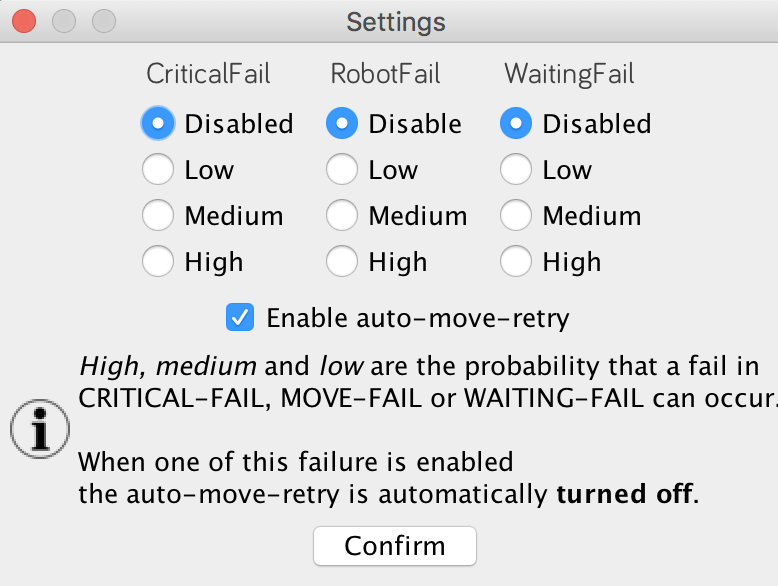
\includegraphics[scale=0.25]{immagini/settings.png}
	\caption{Impostazioni di sistema utilizzate per simulare i fallimenti.}
\end{figure}
\begin{figure}
	\hspace{-2.5cm}
	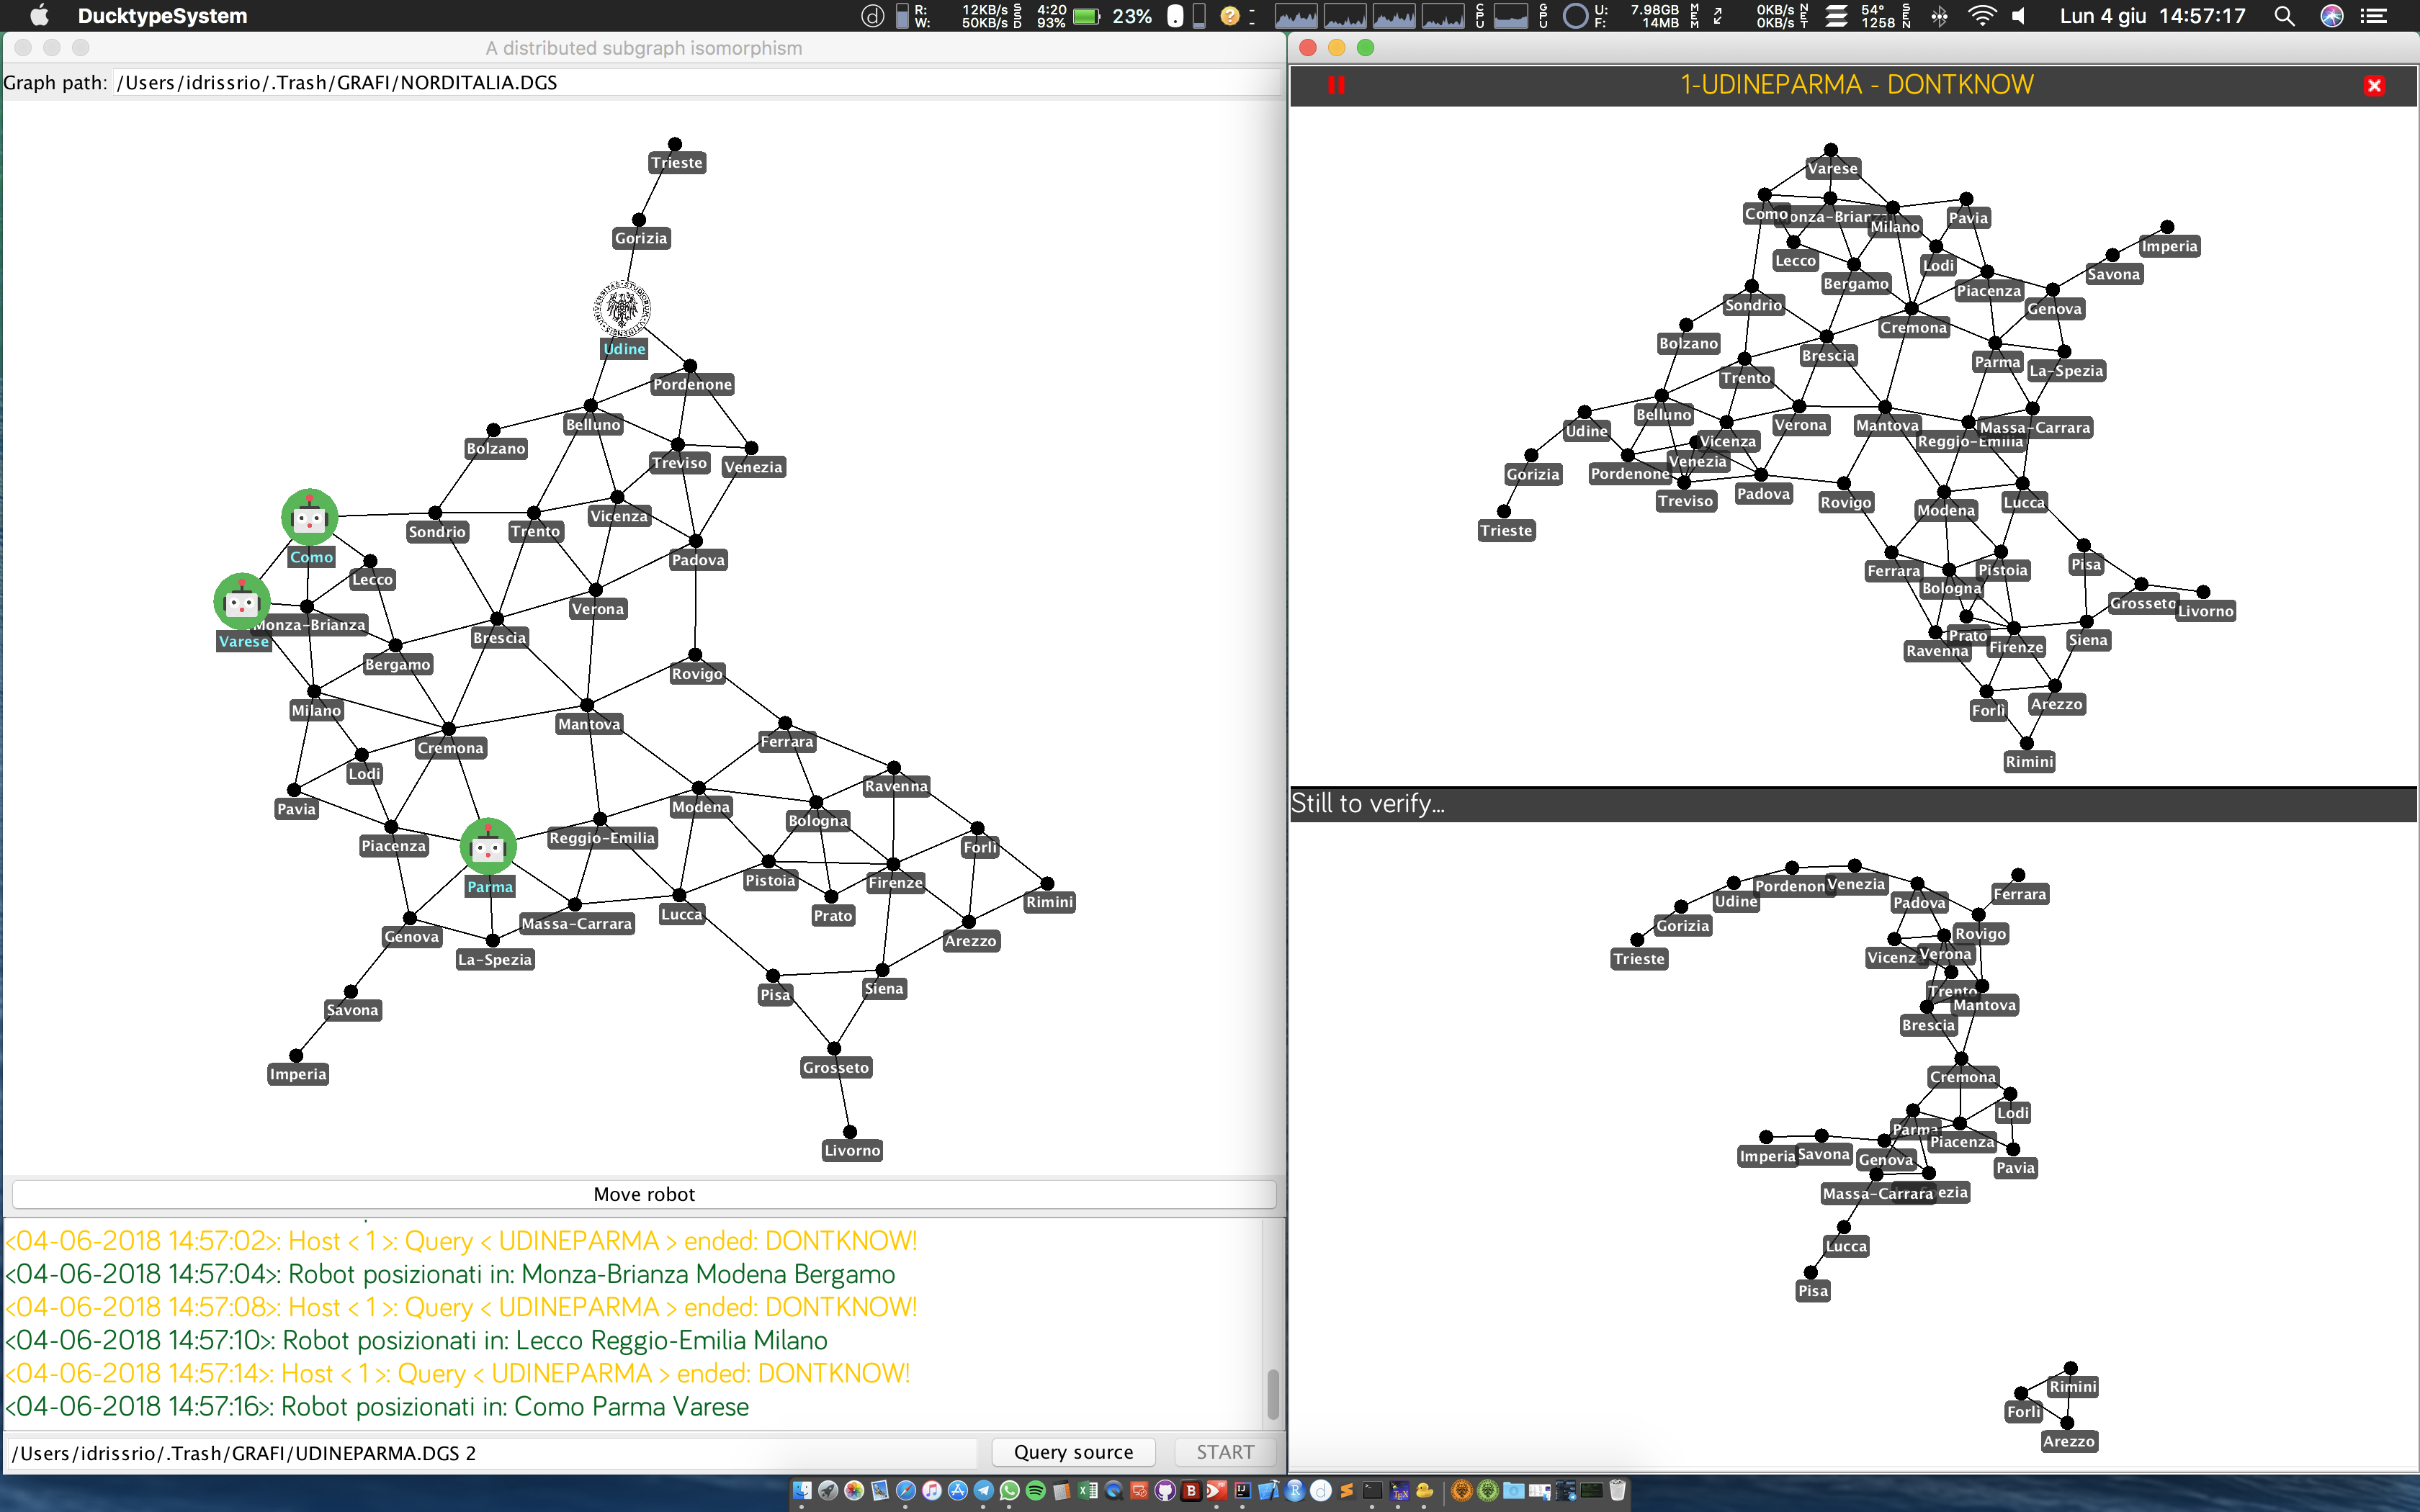
\includegraphics[scale=0.3]{immagini/betterVisualization.png}
	\caption{Modalità \emph{better visualization}: essendo alcuni grafi molto grandi, è stata introdotta la possibilità di scorporare il \emph{JPanel} di destra in una finestra a sè stante, permettendo una migliore visualizzazione delle query.}
\end{figure}




\end{document}
